\documentclass[12pt]{article}
\usepackage{graphicx}
\usepackage{amsmath,amssymb}
\usepackage{hyperref}
\textheight 240mm
\textwidth  170mm
\oddsidemargin  0mm
\evensidemargin 0mm
\topmargin -20mm
\usepackage{listings}
\lstset{
	basicstyle=\ttfamily,,
	xleftmargin=1em
}
\hypersetup{
    colorlinks,
    linkcolor={black},
    citecolor={black},
    urlcolor={black}
}

\begin{document}                                   
%_________________________________________________________________
\title{Project Proposal  - Music Genre Classification\\}
\author{Krishna Chaitanya Sripada, Siva Palakurthi, Soumyatha Gavvala}
\maketitle
%_________________________________________________________________
\section{Introduction}
%_________________________________________________________________
\begin{flushleft}
The rapid growth of the digital media in the past decade has made it easier for man to associate with his interests at a faster and effortless ways. Man has been finding new ways to make music, find, store it and organize it. Finding music was difficult without the name or lyrical content and this lead to the necessity of searching music by its content. Music Information Retrieval (MIR), which is extraction of information about the music from the raw data is a small but fast growing field of research in the similar application. MIR deals with analyzing, creating and categorizing music.\\
\vspace{0.5em}
Our project's aim is to classify a vast collection of musical tracks by their content into different genres. We have taken 729 tracks of known labels as the training data on the basis of which we build the algorithm to categorize unknown test music files. These files were acquired from the website of the 5th International Conference on Music Information Retrieval. These 729 songs belong to six genres.\\
\vspace{0.5em}
\begin{itemize}
\item Classical: 320 songs
\item Electronics: 115 songs
\item Jazz/blues: 26 songs
\item Metal/punk: 45 songs
\item Rock/pop: 101 songs
\item World: 122 songs
\end{itemize}
For the classification of the raw training data given to us, we are using MATLAB as the platform for our algorithms. We are provided with a Music Analysis (MA) toolbox to process the songs which are Pulse Code Modulated and sample them into data that is easier to handle on MATLAB.\\
\vspace{0.5em}
The issue we face is the large size of the data and the classification into genres based on the content which requires the analysis of features of the songs like bandwidth and spectral roll-off. When the songs are converted into matrices, we get a data set of high dimensions and so in order to make it easier to work on the data, we reduce the dimensionality of the data. Then we classify them into groups according to their labels based on the distances between the songs. The distance between two songs of the same genre would be less than that of two songs of different genres. On this basis we cluster the training set into groups thus building an algorithm to classify unknown music files.
\end{flushleft}
%_________________________________________________________________
\section{Distance in song-space}
\begin{flushleft}
For the categorization of these 729 songs into their respective labels, we need an appropriate basis to differentiate them. This we do by measuring the distance between the songs. The distance between two songs of the same genre would be less than that of two songs of different genres. The distance in question is the L2 or Euclidean distance, which is the difference in the sum of squared terms between two given vectors.\\
\vspace{0.5em}
One of the method we have implemented is the calculation of Frobenius norm of the L2 norm. Frobenius norm is also called as Euclidean norm but is not L2 norm. The Frobenius norm of different songs was compared to measure the distance between them.\\
\begin{figure}[!htb]
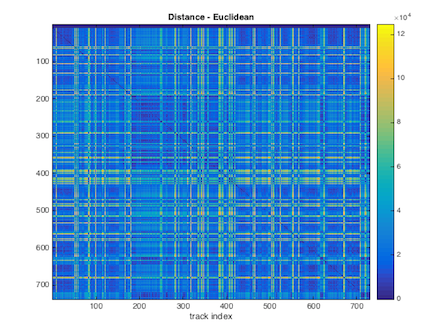
\includegraphics{distance.png}
\caption{Graphical representation of the distance matrices we used. Dark blue regions represent songs which are close to one another while the yellow regions represent a larger distance between songs.}
\end{figure}
\end{flushleft}
%_________________________________________________________________
\section{Dimension reduction}
%_________________________________________________________________
\begin{flushleft}
For the analysis of the training data we need to sample the given songs. We get hundreds of thousands of samples and the dimension of a song in its raw form is huge and impractical to work with directly. So we used several dimensionality reduction techniques in order to reduce the data to dimensions that allowed us to work with the hundreds of songs in the training data set.\\
\subsection{MFCC}
Mel Frequency Cepstral Coefficients (MFCCs), are a pre-processing technique that is frequently used in speech recognition and has been adapted for music information retrieval. The raw data when sampled has dimensions in terms of thousands and it is a strenuous procedure to analyze data of such high dimensions. Due to the high number of samples, the data in each sample is not sufficient for analysis. Hence we requires some pre-processing of the data in order to extract useful information.\\
\vspace{0.5em}
From the MA toolbox provided to us, we make use of the MFCC function to obtain MFC coefficients. These coefficients extract information from songs that is similar to how the human ear hears music that is the content. We first transform the songs into their MFCC coefficients, effectively reducing the dimension of each song while retaining useful information.
\subsection{Principal Component Analysis}
Principal Component Analysis is a statistical procedure that uses an orthogonal transformation to convert a set of observations of possibly correlated variables into a set of values of linearly uncorrelated variables called principal components.\\
\vspace{0.5em}
PCA                     ~\cite{PCA} also called the K-L method searches for \textit{k} \textit{n}-dimensional orthogonal vectors that can best be used to represent the data where k $\leq$n. The original data are thus projected onto a much smaller space resulting in dimensionality reduction. For our experiments, the results of MFCC are passed through the PCA technique which even further reduced the dimension of the songs. The implementation is provided at the end of this document.

\end{flushleft}
%_________________________________________________________________
\section{Statistical learning}
%_________________________________________________________________
\begin{flushleft}
Once the data has been sufficiently reduced in dimension, we used the K-Nearest Neighbors statistical learning method to classify the songs according to their genre. The results of the experiments are provided below.
\vspace{0.5em}
\subsection{K-Nearest Neighbors}
The kNN algorithm               ~\cite{KNN} simply computes the k nearest neighbors to the song which is to be classified, where k $\in$ N is a natural number. The song is then classified into a genre based on the genre of its nearest neighbors. To avoid ties, k is usually chosen to be an odd number.\\
\vspace{0.5em}
This is one of the simplest algorithms and fastest available and can be easily applied to any of our distance matrices by simply sorting the matrix to find the nearest neighbors.
\end{flushleft}
%_________________________________________________________________
\section{Initial Results (extra credit)}
%_________________________________________________________________
\begin{flushleft}
We ran the k-Nearest Neighbors implementation over the entire dataset. The following are the results of using 90\% of the data as the training set and the remaining 10\% of the data as the testing set.\\
\vspace{0.5em}
\begin{tabular}{ |c|c|} 
 \hline
 \textbf{k} & \textbf{Average Accuracy} \\ \hline
 1 & 63.47\% \\ \hline
 3 & 60.84\% \\ \hline
 5 & 66.50\% \\ \hline
 7 & 62.40\% \\ \hline
 9 & 63.02\% \\ \hline
 11 & 64.19\% \\ \hline
 13 & 63.23\% \\ \hline
 15 & 63.80\% \\ \hline
\end{tabular}
\\
\vspace{0.5em}
We algorithm was run on a average of 10 times for every odd value of \textit{k} from the range of 1 to 15. 
\end{flushleft}
%_________________________________________________________________
\section{Discussion}
%_________________________________________________________________
\begin{flushleft}
From the initial experiments, we see that the accuracy using the \textit{k}NN algorithm falls in the range of 60-66\% for different values of \textit{k}. We understand that this accuracy is attributed to the fact that we used a part of the training data for testing and once the testing data is out, we expect the accuracies to improve. But we believe using our current testing data, the accuracy can be improved and would thus like to explore other dimensionality reduction techniques like Latent Dirichlet Allocation(LDA), spectral techniques such as LLE and Laplacian Eigen Maps. Random projections is also something we would look into. The idea is to find out which technique would best describe the data and yet not lose any valuable information about the song. Also we would like to explore other distance measures such as a mixture of multivariate Gaussian distributions to each song along with K-L divergence.\\
\vspace{0.5em}
Apart from this, we believe providing more features would help the classifier. We would try out some of the features like bandwidth of the song, spectral roll-off, spectral flux and loudness. Also other classifiers like Neural Networks, Random Forest based classification and Spectral Clustering would to looked into to see if we can improve the accuracy of our classification by using either of them.
\end{flushleft}
\begin{thebibliography}{}
\addcontentsline{toc}{chapter}{References}  
\bibitem[1]{PCA} \url{http://lvdmaaten.github.io/drtoolbox/}
\bibitem[2]{KNN} \url{http://www.mathworks.com/matlabcentral/fileexchange/45831-matlab-audio-analysis-library}
\end{thebibliography}
\section{Source Code}
\begin{flushleft}
\begin{enumerate}
\item Distance in Song Space
\lstinputlisting[breaklines]{../distance_song_space.m}
\item MFCC and PCA calculation
\lstinputlisting[breaklines]{../main.m}
\lstinputlisting[breaklines]{../DimensionReduction.m}
\item \textit{k}NN classification
\lstinputlisting[breaklines]{../data_conversion_classify_final.m}
\lstinputlisting[breaklines]{../classify.m}
\lstinputlisting[breaklines]{../findPosition.m}
\end{enumerate}
\end{flushleft}
\end{document}
